\head{Апрель}{Листок 7. Графы.}

\begin{thm} \label{7.0 thm1}
    Между 9 планетами Солнечной системы введено космическое сообщение. Ракеты летают по следующим (туда и обратно) маршрутам: Земля - Меркурий, Плутон - Венера, Земля - Плутон, Плутон - Меркурий, Уран - Нептун, Сатурн - Юпитер, Меркурий - Венера, Нептун - Сатурн, Юпитер - Марс и Марс - Уран. Можно ли добраться с Земли до Марса?
\end{thm}

{\setlength{\intextsep}{2pt}
\begin{figure}[h]
\begin{minipage}{0.8\linewidth}\setlength{\parindent}{1.5em}
\begin{thm} 
    На шахматной доске $3 \times 3$ стоят два чёрных и два белых коня (см. рис.). Как поменять чёрных и белых коней местами за наименьшее число ходов? Докажите, что число ходов не может быть меньше найденного. 
\end{thm}
\begin{thm}
    Заменим одного из чёрных коней из предыдущей задачи на красного. Как теперь поменять чёрного и красного коней местами? За какое число ходов это можно сделать?
\end{thm}
\end{minipage}
\hfill
\begin{minipage}{0.17\linewidth}
    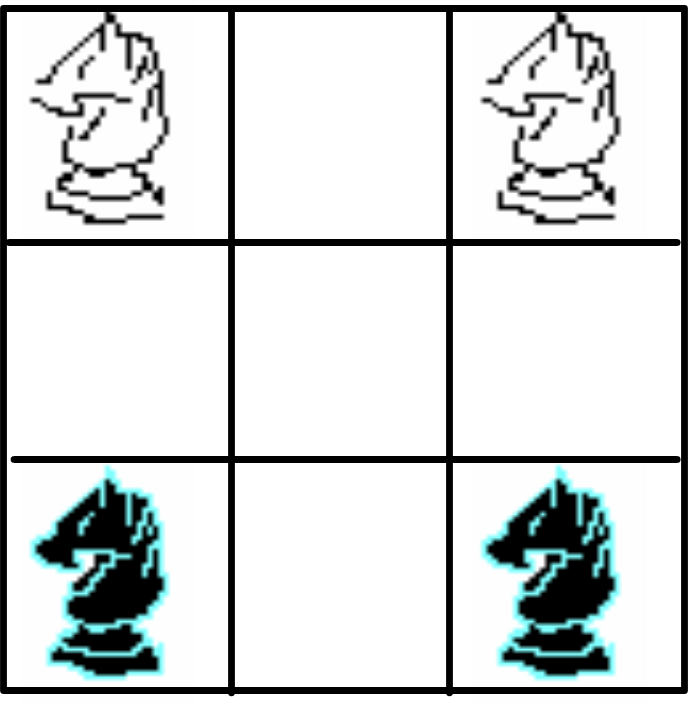
\includegraphics[width=0.9\columnwidth]{img/knight1.png}
\end{minipage}
\end{figure}}

{\setlength{\intextsep}{2pt}
\begin{figure}[h]
\begin{minipage}{0.8\linewidth}\setlength{\parindent}{1.5em}
\begin{thm} $^*$
    На шахматной доске $4 \times 3$ стоят три чёрных и три белых коня (см. рис.) Как поменять чёрных и белых коней местами? $^{**}$ Каково наименьшее число ходов?
\end{thm}
\begin{dfn} \textit{Графом} называется конечное множество точек на плоскости, некоторые пары которых соединены линиями. Эти точки называются \textit{вершинами} графа, а линии - \textit{рёбрами} графа.
\end{dfn}
\par
\begin{dfn} Граф, у которого каждое ребро имеет направление, называется ориентированным графом.
\end{dfn}
\end{minipage}
\hfill
\begin{minipage}{0.17\linewidth}
    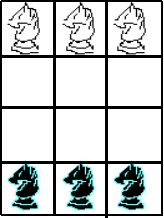
\includegraphics[width=0.9\columnwidth]{img/knight2.png}
\end{minipage}
\end{figure}}

\begin{thm}
    Выпишите в ряд цифры от 1 до 9 так, чтобы любое число, составленное из двух соседних цифр в том же порядке, делилось либо на 7, либо на 13.
\end{thm}

\begin{thm}
    а) В стране Цифра есть 9 городов с названиями 1, 2, 3, 4, 5, 6, 7, 8, 9. Путешественник обнаружил, что из одного города можно долететь самолётом в том и только в том случае, если двузначное число, составленное из цифр-названий городов, при делении на 5 даёт остаток 1. Можно ли добраться из города 1 в город 9? б) Как изменится решение задачи, если города соединены авиалинией в том и только в том случае, когда двузначное число, составленное из названий городов, делится на 3?
\end{thm}

Заметим, что изобразить условие каждой из приведенных выше задач можно с помощью различных графов. Но любой из них поможет нам. Важно лишь, какие именно вершины соединены друг с другом, а какие - нет. Такие ''одинаковые'', но по-разному нарисованные графы называют \textit{изоморфными}.

\begin{ex} \label{7.0 ex1}
    Определите, какие из нарисованных ниже графов изоморфны:
\par
    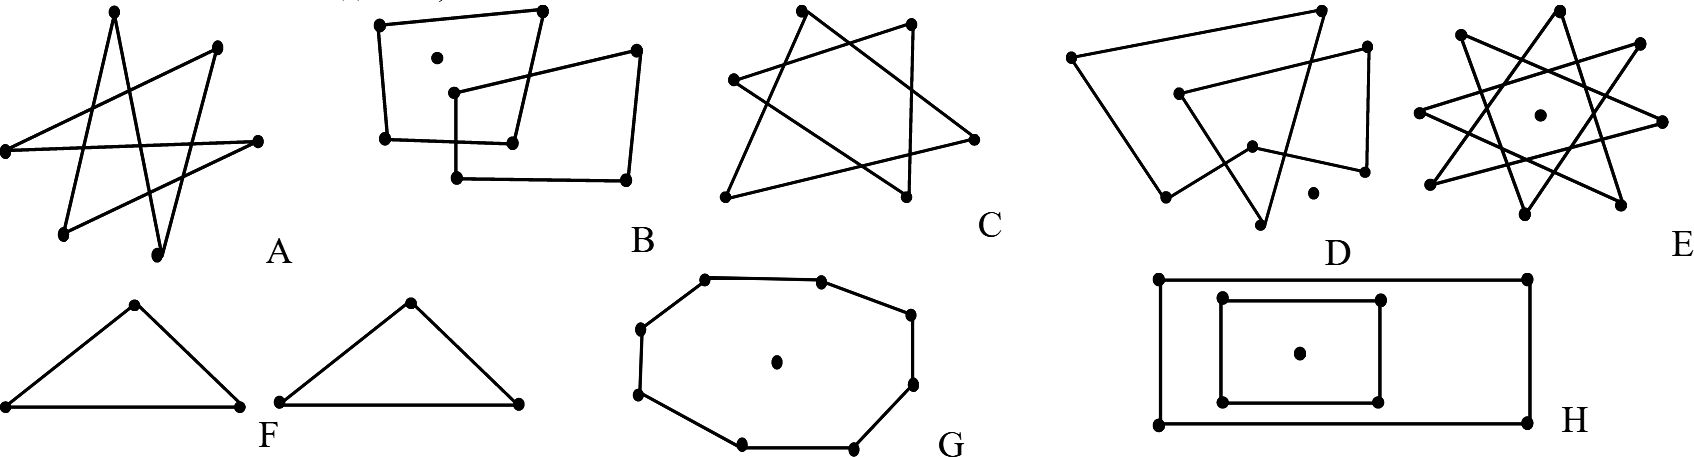
\includegraphics[width=0.95\columnwidth]{img/shapies.png}
\end{ex}

\begin{ex} 
    Нарисуйте по крайней мере три изоморфных графа, соответствующих условию задачи (\ref{7.0 thm1}).
\par
    Мы будем считать, что каждое ребро соединяет различные вершины (нет петель), а каждые две вершины соединены не более чем одним ребром (нет кратных рёбер).
\end{ex}

{\setlength{\intextsep}{2pt}
\begin{figure}[h]
\begin{minipage}{0.8\linewidth}\setlength{\parindent}{1.5em}
\begin{dfn}
    Количество рёбер, выходящих из данной вершины, называется \textit{степенью} этой вершины. Вершина графа, имеющая нечётную степень, называется \textit{нечётной}, а имеющая чётную степень - \textit{чётной}.
\end{dfn}
\begin{ex}
    Укажите степени всех вершин, изображённых на рисунке справа. Сколько здесь чётных вершин, сколько нечётных?
\end{ex}
\end{minipage}
\hfill
\begin{minipage}{0.17\linewidth}
    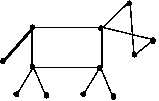
\includegraphics[width=1\columnwidth]{img/loshadka.png}
\end{minipage}
\end{figure}}

\begin{thm} \label{7.0 thm2}
    Известны степени всех вершин графа. Выведите формулу для подсчёта количества рёбер в этом графе.
\end{thm}

\fbox{\begin{minipage}{0.95\textwidth}
    \begin{thrm} \label{7.0 thrm1}
        Число нечётных вершин любого графа чётно.
    \end{thrm}
\end{minipage}} 

\begin{thm} Докажите теорему \ref{7.0 thrm1}.
\par
    Заметим, что задачу \ref{7.0 thm2} часто называют \textit{леммой о рукопожатиях}. Почему? Попробуйте решить такую задачу: ''Докажите, что количество человек, когда-либо живших на земле и сделавших за свою жизнь нечётное число рукопожатий - чётно.'' Что общего между этой задачей и теоремой \ref{7.0 thrm1}? Чему равно количество всех рукопожатий?
\end{thm}

\begin{thm}
    Программисты одного НИИ решили соединить имеющиеся у них 2003 компьютера проводами так, чтобы каждый компьютер был соединен ровно с 3 другими. Удастся ли им осуществить свою идею?
\end{thm}

\begin{prf}
    Если бы это было возможно, то можно было нарисовать граф, где вершины являлись бы изображением компьютеров, а рёбра - проводами. Тогда нарисованный граф имел бы 2003 нечётные вершины, что по лемме о рукопожатиях невозможно.    
\end{prf}

    \begin{ex}
        Переформулируйте на языке графов задачу \ref{1.30} из главы 1 ''Четность''.
    \end{ex}

\begin{ex}
    Переформулируйте на языке графов задачу \ref{2.3 thm2.33} из главы 2 ''Принцип Дирихле''.
\end{ex}

\begin{thm}
    Докажите, что если в графе не менее двух вершин, то в нём есть вершины одинаковой степени.
\end{thm}

\begin{thm} $^*$
    У Маши 24 одноклассника, причём все они имеют различное число друзей в этом классе. Сколько из них дружат с Машей?
\end{thm}

\begin{thm} \label{7.0 thm3}
    В стране Семёрка 15 городов, каждый из которых соединён дорогами не менее, чем с 7 другими. Докажите, что из любого города можно добраться до любого другого (возможно, через другие города).
\end{thm}

\begin{dfn}
    Путём в графе называется последовательность рёбер, каждое следующее из которых начинается в конце предыдущего, последовательность проходимых при этом вершин от $A$ до $B$ также называется \textit{путём, соединяющим вершины $A$ и $B$}.\footnotemark 
\end{dfn}\footnotetext{Вообще говоря, проходимые при этом вершины и рёбра не обязаны быть различными. Путь, в котором никакие вершины и рёбра не встречаются два раза, называют \textit{простым путём}. В данном же листке мы пока не будем выделять различные виды путей.}

\begin{dfn}
    Граф называется связным, если любые его две вершины могут быть соединены путём.
\end{dfn}

Таким образом, решение задачи \ref{7.0 thm3} есть доказательство того, что граф дорог страны Семерка связен. Если граф несвязен, то в нём можно выделить \textit{компоненты связности}, т.е. ''куски'', являющиеся связными графами. Если таких кусков нельзя выделить меньше двух, то граф будет \textit{двухсвязным}, если три, то - \textit{трёхсвязным} и т.д.

\begin{ex}
Укажите число компонент связности для графов из упражнения \ref{7.0 ex1}.
\end{ex}

\begin{thm}
    Верно ли, что любая последовательность рёбер, в которой каждые два имеют общий конец, является путем?
\end{thm}

\begin{thm}
    В графе $n$ вершин. Степень каждой из них не меньше $\dfrac{n - 1}{2}$. Докажите, что граф связен.
\end{thm}

\begin{dfn}
    Замкнутый путь (т.е. путь, у которого совпадают начало и конец), не проходящий через одну вершину дважды, называется \textit{циклом}.
\end{dfn}

\begin{thm}
    На кружок ходит 20 школьников. Однажды им было задано на дом 20 задач. Оказалось, что каждый школьник решил ровно две задачи, а каждую задачу решило ровно два школьника. Докажите, что можно так организовать разбор задач, что каждый школьник расскажет по одной из решенных им задач и все задачи будут разобраны.
\end{thm}

\fbox{\begin{minipage}{0.95\textwidth}
    \begin{thrm} \label{7.0 thrm2}
        Если из каждой вершины конечного графа выходит ровно два ребра, то такой граф является либо циклическим, либо объединением циклических.
    \end{thrm}
\end{minipage}} 

\begin{thm}
Докажите теорему \ref{7.0 thrm2}.
\end{thm}

\begin{thm}
    а) Каково необходимое условие, чтобы у графа можно было обойти все рёбра ровно по одному разу? б) и вернуться в исходную вершину?
\end{thm}

\begin{thm}
    а) Можно ли из одного куска проволоки согнуть каркас куба, не проходя ни по одному ребру дважды? б) А каркас октаэдра? (\textit{Замечание}: октаэдр представляет собой две четырёхугольные пирамиды, склеенные основаниями.)
\end{thm}

\begin{dfn}
    Граф называется \textit{эйлеровым}, если в нём существует замкнутый путь, проходящий через все рёбра ровно по одному разу. Такой путь, соответственно, называют \textit{эйлеровым циклом}.
\end{dfn}

\begin{ex}
    Приведите примеры эйлеровых графов.
\end{ex}        

\textit{Замечание.} Вообще говоря, пути и циклы без самопересечений называют \textit{простыми}. В частности приведенное выше определение цикла есть определение \textit{простого цикла}. Чаще всего в задачах, говоря о циклах, имеют в виду простые циклы.

\begin{ques}
    Верно ли, что эйлеров цикл не имеет самопересечений, то есть всегда является простым циклом?
\end{ques}


\begin{thm} $^*$
    В одном городе на каждом перекрёстке сходится чётное число улиц. Известно, что с любой улицы можно проехать на любую другую. Докажите, что можно объехать все улицы города, побывав на каждой ровно один раз.    
\end{thm}

\begin{thm} $^n$
    В стране Миллениум некоторые города связаны между собой авиалиниями. Из столицы выходит 2007 авиалиний, из города Тьма-Таракань - одна, а из всех остальных городов - ровно по 2008 авиа-линии. Можно ли из Тьмы-Таракани добраться в столицу?
\end{thm}

\begin{thm} $^n$
    Может ли в государстве, в котором из каждого города выходит 3 дороги, быть ровно 100 дорог?
\end{thm}

\begin{thm}
    В стране Стодорожной из каждого города выходит ровно 100 дорог и из любого города можно проехать в любой другой. Одну из дорог закрыли на ремонт. Докажите, что и теперь можно добраться из любого города в любой другой.
\end{thm}

{\setlength{\intextsep}{2pt}
\begin{figure}[h]
\begin{minipage}{0.62\linewidth}\setlength{\parindent}{1.5em}
\begin{thm} $^*$
    Коротышки, проживающие в Цветочном городе, вдруг стали болеть гриппом. В один и тот же день несколько коротышек простудились и заболели, и, хотя потом уже никто не простужался, здоровые коротышки, навещая своих больных друзей, заболевали на следующий день после посещения. Известно, что каждый коротышка болеет гриппом ровно 1 день, причём после этого у него по крайней мере ещё один день есть иммунитет, т.е. он здоров и заразиться в этот день не может (число дней иммунитета у каждого коротышки может быть своё). Несмотря на эпидемию, каждый здоровый коротышка ежедневно навещает всех своих больных друзей. Когда началась эпидемия, коротышки забыли о прививках и не делали их.
\end{thm}
\end{minipage}
\hfill
\begin{minipage}{0.37\linewidth}
    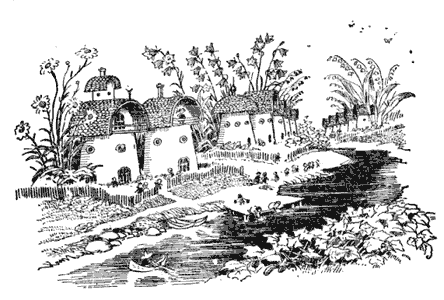
\includegraphics[width=1\columnwidth]{img/houses.png}
\end{minipage}
\end{figure}}
Докажите, что:
\par
а) если до первого дня эпидемии какие-нибудь коротышки сделали прививку и имели в первый день иммунитет, то эпидемия может продолжаться сколь угодно долго;
\par
б) если же в первый день иммунитета ни у кого не было, то эпидемия рано или поздно закончится.

\begin{thm} $^{**}$
    В Простоквашинской начальной школе учится 20 детей. У любых двух из них есть общий дед. Докажите, что тогда найдется Простоквашинский дедушка, у которого в этой школе учится не менее 14-ти внуков и внучек. (Замечание: человек не может иметь более двух дедушек.)
\end{thm}

\newpage

\section{Аналогии.}

И снова старый добрый раздел. Как обычно, вам не нужно пытаться решить \textit{ВСЕ} задачи этого раздела. Необходимо указать все аналогичные задачи, после чего решить одну (если аналогичная задача не была решена ранее) из них на выбор. В этот раз мы постарались вас запутать, изменив числовые данные в задачах, поэтому задачи могут быть аналогичны друг другу, даже имея различные числовые данные.

\begin{thm}
    В лицее 55 кабинетов. Хакер Макс решил соединить телефонными проводами каждый кабинет ровно с пятью другими. Сможет ли он это сделать?
\end{thm}

\begin{thm}
    Во дворе живут 4 пёсика: Бобик, Робик, Тобик и Толстолобик. Каждому из них случалось драться с кем-нибудь из остальных, причём у Бобика, Робика и Тобика число тех, с кем они дрались - разное. Со сколькими собаками двора дрался Толстолобик?
\end{thm}

\begin{thm}
    Докажите, что среди девяти человек найдутся либо трое попарно знакомых, либо четверо попарно незнакомых.
\end{thm}

\begin{thm}
    На плоскости нарисованы 9 точек. Костя соединил некоторые из них синим цветом, а Миша все остальные точки соединил красным. Докажите, что найдётся либо синий треугольник, либо красный четырёхугольник с красными диагоналями.
\end{thm}

\begin{thm}
    В сказочной стране Перра-Терра живут карабасы и барабасы. Каждый карабас знаком с 4 барабасами и 7 карабасами, а каждый барабас знаком с 6 карабасами и 5 барабасами. Кого в стране больше - карабасов или барабасов?
\end{thm}

\begin{thm}
    Можно ли нарисовать на плоскости 9 отрезков так, чтобы каждый пересекался ровно с тремя другими?
\end{thm}

\begin{thm}
    Проходит волейбольный турнир школы по круговой системе (каждая команда играет с каждой ровно один раз). Участвует 17 команд. В том числе и команда 7Ю класса. В некоторый момент времени оказалось, что все команды (кроме команды 7Ю) сыграли разное количество матчей. Сколько матчей к этому моменту сыграла команда 7Ю класса? 
\end{thm}

\begin{thm}
    В кружке танцев каждая девочка познакомилась с 6 мальчиками и 7 девочками, а каждый мальчик - с 3 девочками и 4 мальчиками. Кого в кружке больше: мальчиков или девочек?
\end{thm}

{\setlength{\intextsep}{2pt}
\begin{figure}[h]
\begin{minipage}{0.62\linewidth}\setlength{\parindent}{1.5em}
\begin{thm}
    Резидент одной из иностранных разведок сообщил, что пятнадцать республик бывшего Советского Союза заключили несколько двусторонних соглашений так, что каждая из них заключила договор ровно с тремя другими. Заслуживает ли резидент доверия?
\end{thm}

\begin{thm}
    Докажите, что на любой географической карте с 2008 странами найдутся по крайней мере две страны с одинаковым числом соседей.
\end{thm}

\begin{thm}
    В государстве $N$ ровно $2n + 1$ городов. Новый президент издал указ, по которому каждый город должен быть соединён автострадой ровно с $2k + 1$ другими. Для каких значений $n$ и $k$ можно выполнить указ президента?
\end{thm}
\end{minipage}
\hfill
\begin{minipage}{0.37\linewidth}
    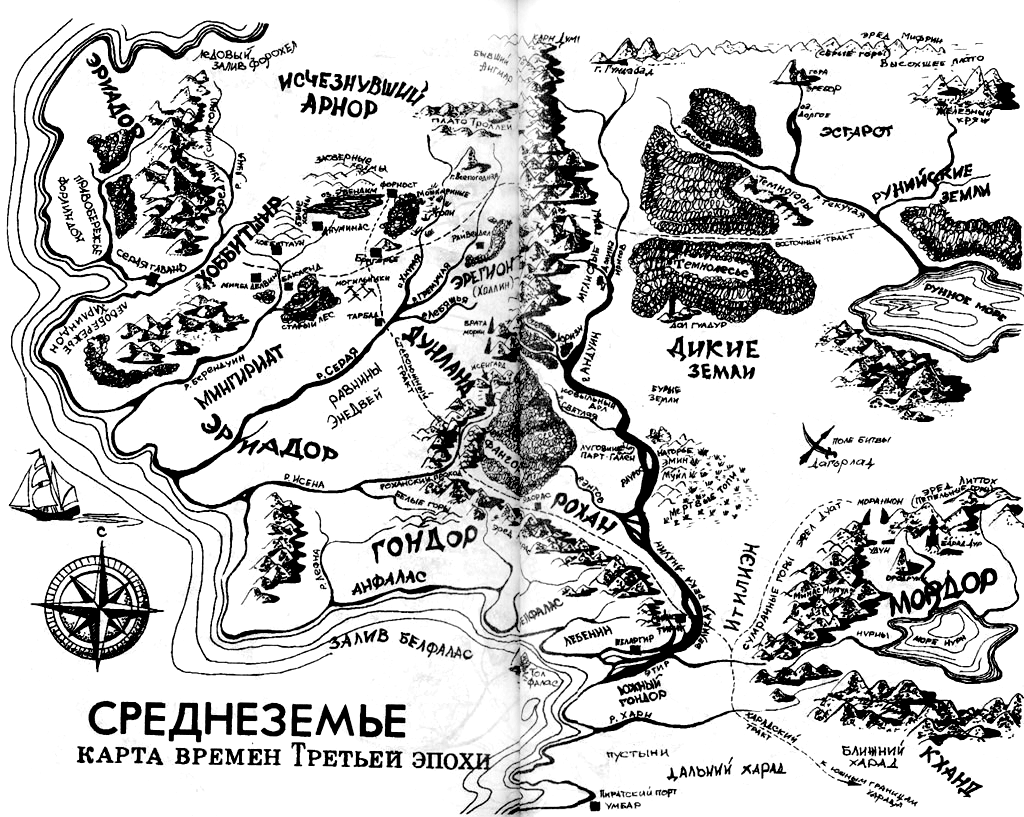
\includegraphics[width=1\columnwidth]{img/map.png}
\end{minipage}
\end{figure}}

\begin{thm}
    В стране Девятка девять городов. Некоторые из них соединены авиалиниями (туда и обратно). Докажите, что либо найдутся три города, которые можно облететь по циклу, либо четыре города, никакие два из которых не соединены авиалинией.
\end{thm}

\begin{thm}
    В графе каждая вершина покрашена в синий или зелёный цвет. При этом каждая синяя вершина связана с пятью синими и десятью зелёными, а каждая зелёная с девятью синими и шестью зелёными. Каких вершин больше - синих или зелёных?
\end{thm}

\newpage

\section{Дополнительные задачи.}

\begin{thm}
    На шахматной доске $4 \times 4$ расположена фигура - ''летучая ладья'', которая ходит так же как и обычная ладья, но не может за один ход стать на поле соседнее с предыдущим. Может ли она обойти всю доску, становясь на каждое поле по одному разу и вернуться на исходное поле?
\end{thm}

\begin{thm}
    В Тридевятом царстве любые два города соединены дорогой с односторонним движением. Докажите, что существует город, из которого можно добраться в любой другой не более, чем по двум дорогам.
\end{thm}

\begin{thm} $^*$
    В одном городе любые двое - либо друзья, либо враги. Каждый человек может в некоторый момент поссорится со всеми своими друзьями и помириться со всеми своими врагами. Оказалось, что таким образом любые трое могут стать друзьями. Докажите, что тогда и все люди в этом городе могут стать друзьями.
\end{thm}

\begin{thm} $^*$
    В стране 201 город, из каждого выходит ровно 10 дорог, причем из любого города можно доехать до любого другого. Докажите, что можно выбрать 20 городов, никакие два из которых не соединены дорогой.
\end{thm}

\begin{thm} $^*$
    На турбазе 12 домиков, между которыми крот прокопал 56 непересекающихся подземных ходов (два домика соединяются не более чем одним ходом). Докажите, что крот из любого домика может попасть в любой другой, передвигаясь по этим ходам.
\end{thm}

\begin{thm} $^*$
    Можно ли сетку, состоящую из границ единичных квадратиков клетчатого квадрата $4 \times 4$, представить в виде объединения 
    \par
    а) восьми ломаных длиной 5;
    \par
    б) пяти ломаных длиной 8?
\end{thm}